\pagestyle{hedra}
\label{hedra}

\begin{textblock*}{5.625in}(0pt,0pt)%
\vspace*{-1.45cm}
\hspace*{-1.2cm}\includegraphics*[width=112mm]{./imgs/HEDRA.png}
\end{textblock*}

\pagebreak


\hspace{.5cm}

\begin{center}
\hspace*{-.5cm}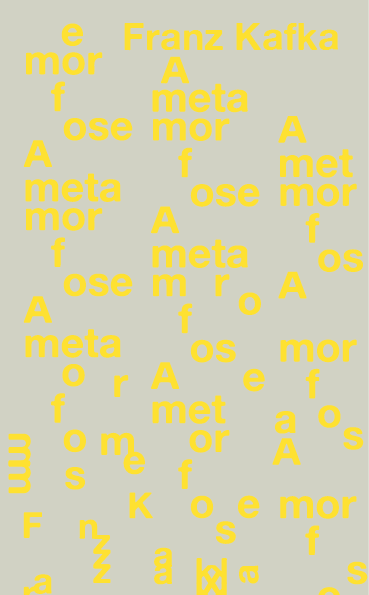
\includegraphics[width=45mm]{./imgs/kafka.png}
\end{center}

\hspace*{-2cm}\_\_\_\_\_\_\_\_\_\_\_\_\_\_\_\_\_\_\_\_\_\_\_\_\_\_\_\_\_\_\_\_\_\_\_\_\_\_\_\_\_\_\_\_\_\_\_\_\_\_\_\_\_\_\_\_\_\_\_\_\_\_\_\_\_\_\_\_\_\_\_\_\_\_

\medskip

\noindent{}Obra mais famosa de Franz Kafka, {\slsc{A metamorfose}} dispensa apresentações. A história da transformação de Gregor Samsa é um clássico porque condensa perfeitamente as características da prosa kafkiana, este conceito que se torna importante na nossa repertoriação do mundo: kafkiano é, pois, o contraditório da nossa cultura ocidental desumanizada, em que o irracional é criado justamente pelas estruturas burocráticas ultrarracionalizadas.

\hspace{.5cm}

\hspace*{-.4cm}\begin{minipage}[c]{0.90\linewidth}
\small{
{\Formular{\textbf{
\hspace*{-.1cm}Título: A metamorfose\\
Autor: Franz Kafka\\ 
Editora: Hedra\\
Páginas: 196\\
Formato: 13x21cm\\
Preço: R\$ 39,90\\
ISBN: 978-85-7715-601-6
}}}}
\end{minipage}


\pagebreak

\hspace{.5cm}

\begin{center}
\hspace*{-2.5cm}\raisebox{5.5cm}{\rotatebox[origin=t]{90}{\Formular{\textbf{Lançamento}}}}
\hspace{2cm}
\includegraphics[width=45mm]{./imgs/maquiavel.png}
\end{center}

\hspace*{-2cm}\_\_\_\_\_\_\_\_\_\_\_\_\_\_\_\_\_\_\_\_\_\_\_\_\_\_\_\_\_\_\_\_\_\_\_\_\_\_\_\_\_\_\_\_\_\_\_\_\_\_\_\_\_\_\_\_\_\_\_\_\_\_\_\_\_\_\_\_\_\_\_\_\_\_

\medskip

\noindent{}{\slsc{O príncipe}} ganha sua mais completa edição bilíngue, trazendo ao leitor brasileiro contato com a melhor edição do texto original italiano --- a Edição Crítica Inglese ---, acrescida de introdução e notas explicativas. Obra mais emblemática de Nicolau Maquiavel, {\slsc{O príncipe}} assinala uma nova forma de analisar a política, marcada principalmente pelo realismo que procura apreender a política como ela é --- em sua prática terrena.

\hspace{.5cm}

\hspace*{-.4cm}\begin{minipage}[c]{0.90\linewidth}
\small{
{\Formular{\textbf{
\hspace*{-.1cm}Título: O príncipe\\
Autor: Nicolau Maquiavel\\ 
Editora: Hedra\\
Páginas: 508\\
Formato: 13x21cm\\
Preço: R\$ 49,90\\
ISBN: 978-85-7715-604-7
}}}}
\end{minipage}

\pagebreak

\hspace{.5cm}

\begin{center}
\hspace*{-.5cm}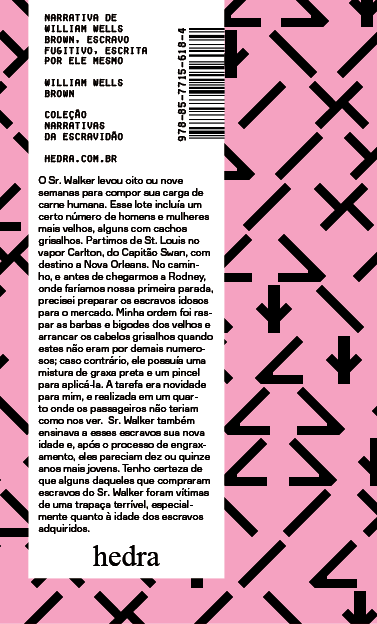
\includegraphics[width=43mm]{./imgs/wwb.png}
\end{center}

\hspace*{-2cm}\_\_\_\_\_\_\_\_\_\_\_\_\_\_\_\_\_\_\_\_\_\_\_\_\_\_\_\_\_\_\_\_\_\_\_\_\_\_\_\_\_\_\_\_\_\_\_\_\_\_\_\_\_\_\_\_\_\_\_\_\_\_\_\_\_\_\_\_\_\_\_\_\_\_

\medskip

\noindent{}Romancista, dramaturgo, historiador e militante abolicionista, William Wells Brown tem em sua {\slsc{Narrativa autobiográfica}} um dos mais importantes romances afro"-americanos da história. A obra reconta os horrores da escravidão, percorrendo o tráfico interno de escravos nos \scalebox{.8}{EUA} e a relação de Brown com seus donos e familiares, destacando assim a individualidade e que se desenvolveu sob uma instituição totalizante e desumanizadora.

\hspace{.5cm}

\hspace*{-.4cm}\begin{minipage}[c]{0.90\linewidth}
\small{
{\Formular{\textbf{
\hspace*{-.1cm}Título: Narrativa de William Wells Brown, escravo fugitivo, escrita por ele mesmo\\
Autor: William Wells Brown\\ 
Editora: Hedra\\
Páginas: 142\\
Formato: 14x21cm\\
Preço: R\$ 39,90\\
ISBN: 978-85-7715-618-4
}}}}
\end{minipage}

\pagebreak

\hspace{.5cm}

\begin{center}
\hspace*{-2.5cm}\raisebox{5.5cm}{\rotatebox[origin=t]{90}{\Formular{\textbf{Lançamento}}}}
\hspace{2cm}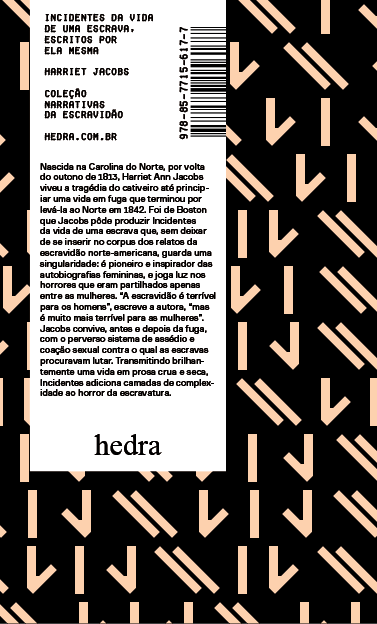
\includegraphics[width=45mm]{./imgs/jacobs.png}
\end{center}

\hspace*{-2cm}\_\_\_\_\_\_\_\_\_\_\_\_\_\_\_\_\_\_\_\_\_\_\_\_\_\_\_\_\_\_\_\_\_\_\_\_\_\_\_\_\_\_\_\_\_\_\_\_\_\_\_\_\_\_\_\_\_\_\_\_\_\_\_\_\_\_\_\_\_\_\_\_\_\_

\medskip

\noindent{}Nascida na Carolina do Norte, por volta do outono de 1813, Harriet Ann Jacobs viveu intensamente a tragédia da escravidão, e dela resulta este relato cru, de prosa vívida e dramática que, sem deixar de se inserir no corpus dos relatos da escravidão norte"-americana, é pioneiro e inspirador das autobiografias femininas, e joga luz no perverso sistema de assédio e coação que era partilhado apenas entre as mulheres.

\hspace{.5cm}

\hspace*{-.4cm}\begin{minipage}[c]{0.90\linewidth}
\small{
{\Formular{\textbf{
\hspace*{-.1cm}Título: Incidentes da vida de uma escrava\\
Autor: Harriet Jacobs\\ 
Editora: Hedra\\
Páginas: 406\\
Formato: 14x21cm\\
Preço: R\$ 59,90\\
ISBN: 978-85-7715-617-7
}}}}
\end{minipage}


\pagebreak

\hspace{.5cm}

\begin{center}
\hspace*{-.5cm}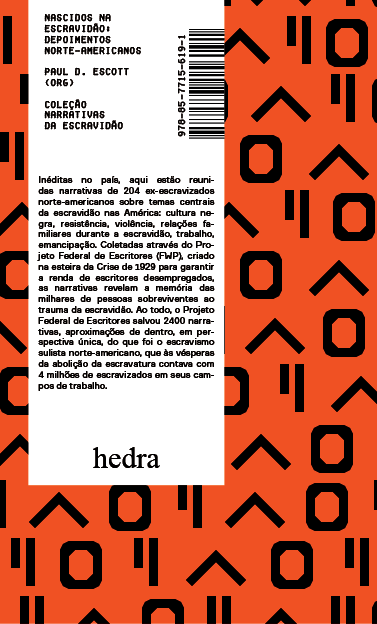
\includegraphics[width=43mm]{./imgs/wpa.png}
\end{center}

\hspace*{-2cm}\_\_\_\_\_\_\_\_\_\_\_\_\_\_\_\_\_\_\_\_\_\_\_\_\_\_\_\_\_\_\_\_\_\_\_\_\_\_\_\_\_\_\_\_\_\_\_\_\_\_\_\_\_\_\_\_\_\_\_\_\_\_\_\_\_\_\_\_\_\_\_\_\_\_

\medskip

\noindent{}{\slsc{Nascidos na escravidão}} resulta de um amplo esforço de tomar depoimentos de ex"-escravos dos Estados Unidos, totalizando 2400 narrativas inéditas, das quais a edição reúne 204, em uma curadoria por tema que permite entrever a memória das milhares de pessoas sobreviventes do trauma do cativeiro, em sua complexidade, e desmontar certos mitos correntes sobre a escravidão através de depoimentos em primeira mão.


\hspace{.5cm}

\hspace*{-.4cm}\begin{minipage}[c]{1\linewidth}
\small{
{\Formular{\textbf{
\hspace*{-.1cm}Título: Nascidos na escravidão: depoimentos norte"-americanos\\
Autor: Paul D. Scott (org.)\\ 
Editora: Hedra\\
Páginas: 348\\
Formato: 14x21cm\\
Preço: R\$ 39,90\\
ISBN: 978-85-7715-619-1
}}}}
\end{minipage}

\pagebreak

\hspace{.5cm}

\begin{center}
\hspace*{-2.5cm}\raisebox{5.5cm}{\rotatebox[origin=t]{90}{\Formular{\textbf{Lançamento}}}}
\hspace{2cm}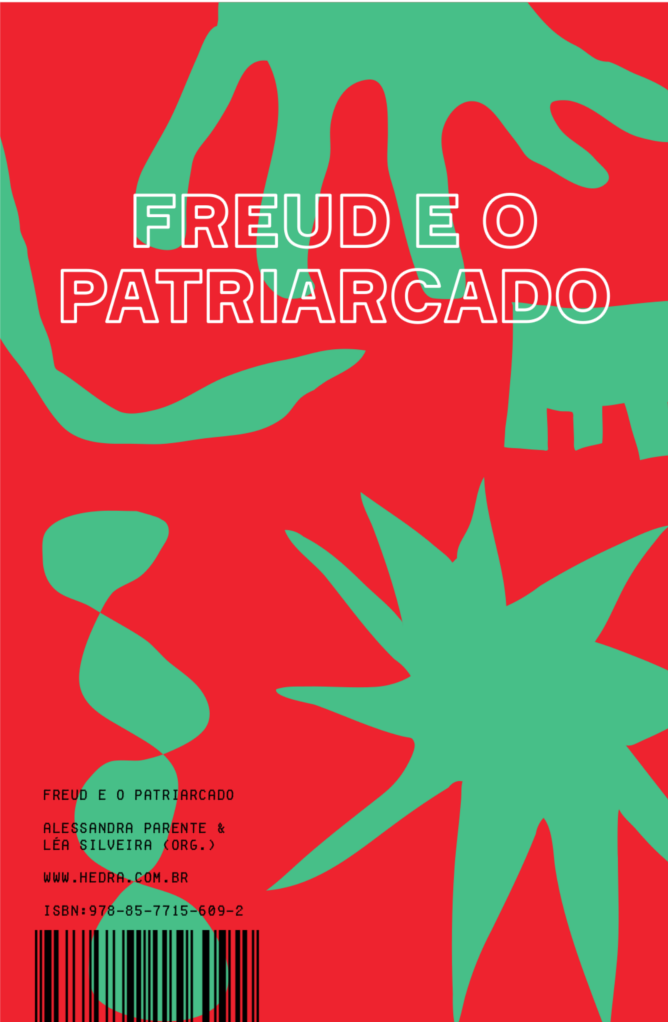
\includegraphics[width=45mm]{./imgs/freud.png}
\end{center}

\hspace*{-2cm}\_\_\_\_\_\_\_\_\_\_\_\_\_\_\_\_\_\_\_\_\_\_\_\_\_\_\_\_\_\_\_\_\_\_\_\_\_\_\_\_\_\_\_\_\_\_\_\_\_\_\_\_\_\_\_\_\_\_\_\_\_\_\_\_\_\_\_\_\_\_\_\_\_\_

\medskip

\noindent{}{\slsc{Freud e o patriarcado}} parte da constatação de que o campo da teoria psicanalítica põe em jogo uma forma de conceber o psíquico que assume, em seu centro, uma equivalência generalizada entre cultura, civilização e masculinidade, algo que, para as autoras e os autores de {\slsc{Freud e o patriarcado}}, deveria ser explicado, não dado. Sobre essa trilha, trata"-se de explorar a legitimidade dos modelos freudianos, seja preservando"-os ou repensando"-os.

\hspace{.5cm}

\hspace*{-.4cm}\begin{minipage}[c]{0.90\linewidth}
\small{
{\Formular{\textbf{
\hspace*{-.1cm}Título: Freud e o patriarcado\\
Autor: Alessandra Parente e Léa Silveira (org.)\\ 
Editora: Hedra\\
Páginas: 398\\
Formato: 16x23cm\\
Preço: R\$ 64,90\\
ISBN: 978-85-7715-611-5
}}}}
\end{minipage}

\pagebreak

\hspace{.5cm}

\begin{center}
\hspace*{-.5cm}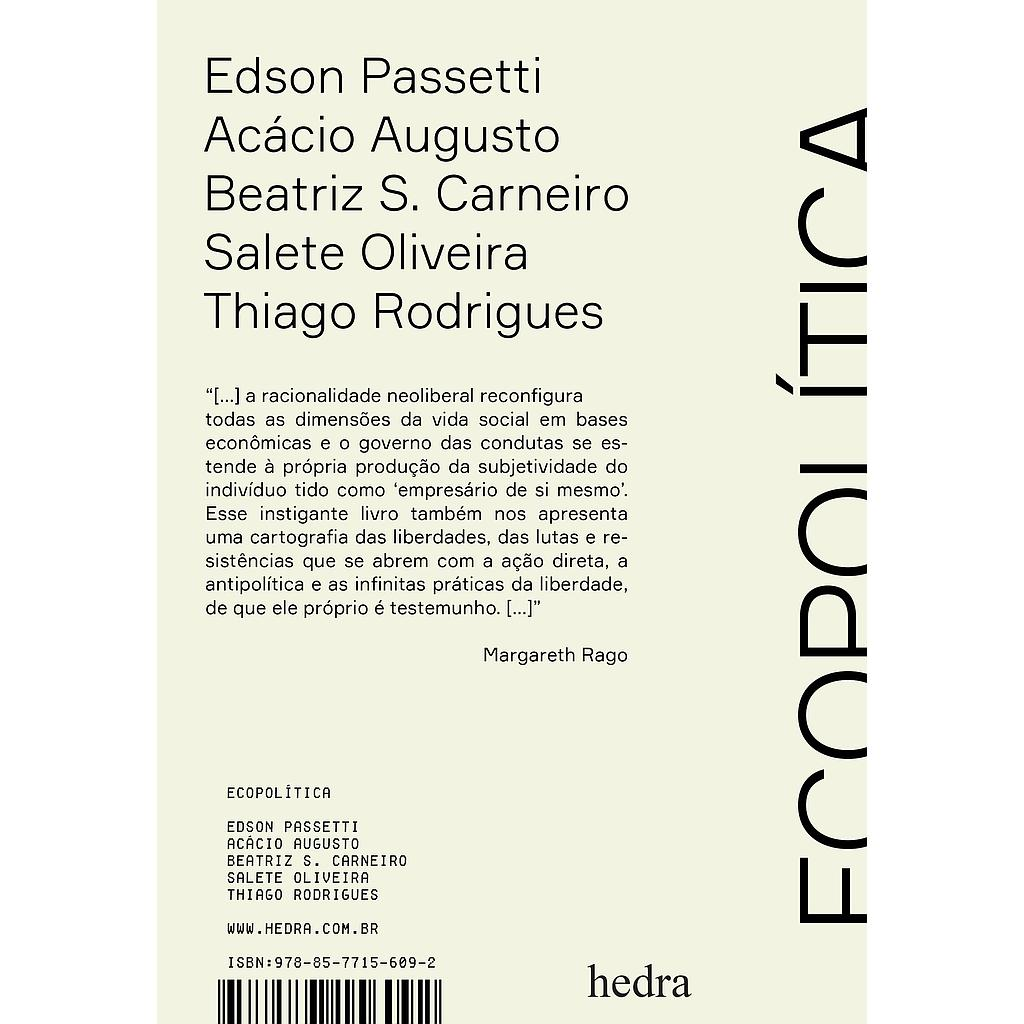
\includegraphics[width=70mm]{./eco.jpeg}
\end{center}

\hspace*{-2cm}\_\_\_\_\_\_\_\_\_\_\_\_\_\_\_\_\_\_\_\_\_\_\_\_\_\_\_\_\_\_\_\_\_\_\_\_\_\_\_\_\_\_\_\_\_\_\_\_\_\_\_\_\_\_\_\_\_\_\_\_\_\_\_\_\_\_\_\_\_\_\_\_\_\_

\medskip

\noindent{}{\slsc{Ecopolítica}} mapeia a passagem da biopolítica — o controle da vida analisado por Foucault — para a ecopolítica, nova forma de governar que emerge pós-\scalebox{.8}{II} Guerra Mundial e se estende a todas as esferas do mundo natural. Os estudiosos do grupo Nu"-Sol percorrem e analisam acontecimentos históricos e contemporâneos, e atravessam fluxos de poder para conclamar à criação de resistências libertárias e esquivas às globalizantes linhas de controle.

\hspace{.5cm}

\hspace*{-.4cm}\begin{minipage}[c]{0.90\linewidth}
\footnotesize{
{\Formular{\textbf{
\hspace*{-.1cm}Título: Ecopolítica\\
Autor: Edson Passetti (org.)\\ 
Editora: Hedra\\
Páginas: 476\\
Formato: 16x23cm\\
Preço: R\$ 79,90\\
ISBN: 978-85-7715-609-2
}}}}
\end{minipage}

\pagebreak